\documentclass[border=5mm,tikz]{standalone}
\usepackage{pgfplots}
\pgfplotsset{compat=1.8}

\usepackage{amsmath}

\pgfplotsset{ % Define a common style, so we don't repeat ourselves
    MaoYiyi/.style={
        width=0.6\textwidth, % Overall width of the plot
        axis equal image, % Unit vectors for both axes have the same length
        view={0}{90}, % We need to use "3D" plots, but we set the view so we look at them from straight up
        xmin=0, xmax=110, % Axis limits
        ymin=0, ymax=110,
        domain=0:100, y domain=0:100, % Domain over which to evaluate the functions
        xtick={0,20,...,100}, ytick={0,20,...,100}, % Tick marks
        samples=11, % How many arrows?
        cycle list={    % Plot styles
                gray,
                quiver={
                    u={1}, v={f(x)}, % End points of the arrows
                    scale arrows=7.5,
                    every arrow/.append style={
                        -latex[white] % Arrow tip
                    },
                }\\
                red, samples=31, smooth, thick, no markers, domain=0:110\\ % The plot style for the function
        }
    }
}

\begin{document}
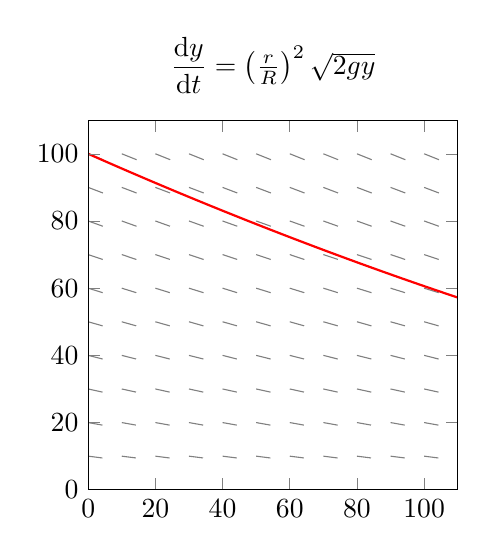
\begin{tikzpicture}[
    declare function={f(\x) = -0.04*sqrt{\y};} % Define which function we're using
]
    \pgfmathsetmacro{\R}{10}
    \pgfmathsetmacro{\r}{1}
    \pgfmathsetmacro{\g}{9.81}
    \pgfmathsetmacro{\h}{100}

\begin{axis}[
    MaoYiyi, title={$\dfrac{\mathrm{d}y}{\mathrm{d}t}=\left(\frac{r}{R}\right)^2\sqrt{2gy}$}
]
%r= \r, R=\R, h=\h
\addplot3 (x,y,0);
\addplot {((sqrt(2*\h) - (\r/\R)^2*sqrt(\g)*x)^2)*0.5}; % You need to find the antiderivative yourself, unfortunately. Good exercise!
\end{axis}
\end{tikzpicture}
%

\end{document} 